\documentclass[12pt]{article}
\usepackage{fullpage,enumitem,amsmath,amssymb,graphicx}

\newcommand{\figcaption}{\def\@captype{figure}\caption} 

\begin{document}

\begin{center}
{\Large Hanabi Game Player}

\begin{tabular}{rl}
\\
&Qian Lin, Shanshan Xu \\
\end{tabular}
\end{center}


\section{Game Dynamics}
Each card is characterized by a pair consisting of color and number.
Each of the $N$ players takes actions sequentially.

\textbf{State:}  Each state contains the following information
\begin{itemize}
\item[$\bullet$] All the cards remaining in the deck. 
\item[$\bullet$] All the cards played in the table.
\item[$\bullet$] All the discarded cards in the trash.
\item[$\bullet$] The cards in each player's hand. Each card also contains the information wether its color and number are known to its owner. 
\item[$\bullet$] The number of clues remained.
\item[$\bullet$] The number of additional terms left. `inf' means the mode of the additional rounds haven't been activated.   
\end{itemize}

\textbf{IsEnd(s):} All the distinct cards appear in the table. Or the number of additional terms is zero.

\textbf{Actions:} Each player can takes one of the following actions unless the condition is not satisfied. At the first time when a player tries to draw a new card from 
the empty deck, the mode of the additional rounds is activated and the number of additional terms is set to be the number of players in the game.
After the turn that the mode of the additional rounds is 
activated, each taken action makes the number of additional terms decreased by one. 
\begin{itemize}
\item[$\bullet$] (`play', $i$):  The player chooses his/her $i$-th card. If there is some card in the table with the same color  but has the number closely 
before this $i$-th card, the card is added in the table. Otherwise, the card is discarded into trash and the number of clues decreases by one if larger than zero. 
Finally, the player draws a new card from the deck if the deck is not empty. 
\item[$\bullet$]  (`discard', $i$): The player discard his/her $i$-th card into the trash. The number of clues increases by one if smaller than the initial value. Finally, 
the player draws a new card from the deck if the deck is not empty. 
\item[$\bullet$] (`color', $p$, $c$): The player tells the $p$-th player which cards in the $p$-th player's hand have the color $c$. This action is allowed only when 
the number of clues is larger than zero. After this action, the number of clues decreases by one.
\item[$\bullet$] (`number', $p$, $n$): The player tells the $p$-th player which cards in the $p$-th player's hand have the number $n$. This action is allowed only when 
the number of clues is larger than zero. After this action, the number of clues decreases by one.
\end{itemize}

\textbf{Succ(s,a):} return a new state from $s$ following the description of the action $a$ in the above. 

\textbf{Utility(s):}  The sum of all the cards' numbers in the table.  

\section{Description of Cards}
\textbf{Card label:} each card is labeled by a tuple (c, n), where c=0,...numColor-1 represents its color, and n=0,...maxNumber-1 represents its number. Depend on the state of the table (cards already played) and the trash (cards discarded), which is common knowledge to all players, a set of properties describes a card whose partial information is known.

\textbf{Definition for playable:} if a card has enough information to be played. For example, if no cards have been played, one card with n = 0 is playable regardless of its color. 

\textbf{Definition for discardable:} if a card has enough information to be judged as a duplicate of a card on the table. 

\textbf{Definition for dangerous:} if a card has enough information to be judged as the only card of its kind left and has not been played.

Discardable has no intersection set with playable or dangerous. However, a card can be simultaneously playable and dangerous. For practical purpose, the playable property takes priority.

\section{Agent State}
Each agent state has the following variables:
\begin{itemize}
 \item cards: a list of cards from oldest to newest. This is known only to the other agents.
 \item know: a list of tuple of binaries indicating whether a property (color, number) of a particular card is known. This is known by all agents (both the owner and the other agents).
 \item infer: a list of inference about card made by the owner about his own cards. The type of information stored in the infer list is agent-type-specific. This is known only to the owner.
\end{itemize}

Besides the getAction() method, each agent also has a inference() method, which takes the gameState, player index and action as input, and updates its AgentState.infer.

\section{Strategies}
The unique feature of Hanabi is that it is a cooperative multi-agent game with incomplete information. Although it is deterministic (in that its successor state is unique) and can technically be described by a game tree, each player may need to have a probabilistic model describing its own viewpoint.

The mainly several challenges we try to address in designing our game agents are

Firstly, what's the appropriate amount of hard-coded heuristics, and how to optimize the set of heuristics. Human Hanabi players uses simple heuristics like always discard the oldest card first or a clue means either play or keep, as well as complicated heuristics such as if only one 1 card is played, a clue informing a card being 1 means play. We will see that some of this complicated heuristics will emerge from our coded agents using only simple heuristics and statistical inference.

Secondly, how to perform effective inference to estimate viewpoints, and how to incorporate recursive inference, previous run clue and multi-agents. This is still undergoing effort.

As we will see below, the random player (no heuristics, no inference) scores 6 out of a 25/50 stack, while the oracle (complete information) scores close to 25 out of 25/50 stack. Reasonably experienced human players can also score an average 24 out of 25/50, and it is our goal to match that score. 

At the moment our agents using simple heuristic or/and one recursive inference achieves an average of 16 out of 25/50. There's still much space to improve as we try to refine our heuristics and implement more sophisticated inference method.

A comparison of the previous five types of agent is plotted below
\begin{figure}[hbt]
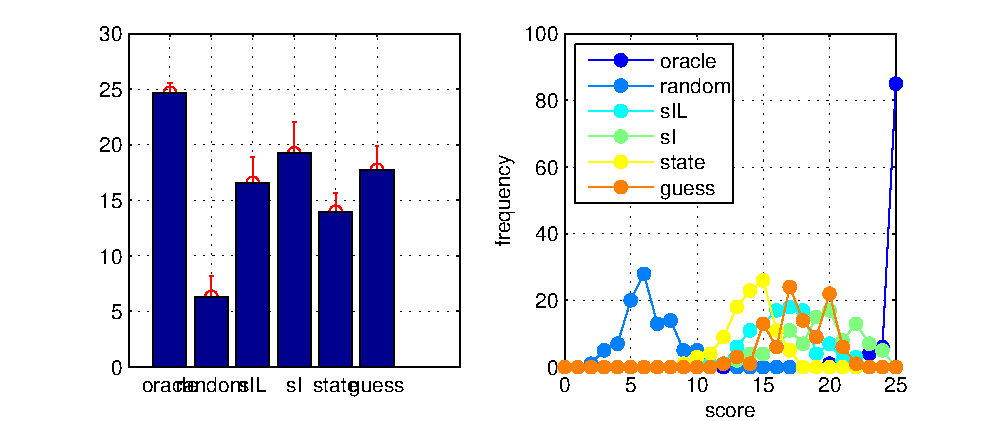
\includegraphics[width=6in]{data/data.pdf}
\caption{Left: mean and stander deviation of scores over 100 trails. Right: histogram of scores over data used in the left plot.}
\end{figure}

\subsection{Random Player (Baseline)}
Each players takes action randomly. The player first randomly chooses the first element of the action  `play', 'discard', 'color', 'number' with probabilities $1/3$, $1/3$, $1/6$, $1/6$, respectively.  Then the left elements in the action are sampled by a uniform distribution. We expect that this strategy gives the lower bound of the utility in this game.

This scores on average 6 out of a 25/50 card stack.

\subsection{Oracle}
If each player knows its own card, then it can always play optimally. This will not guarantee a win, depending on end-game situation. The oracle follows the strategy
\begin{itemize}
 \item play the oldest playable card
 \item if information token is available, spend it
 \item discard the oldest discardable card
 \item discard the oldest non-dangerous card
 \item discard a random card
\end{itemize}
This scores very close to 25 out of a 25/50 card stack.

\subsection{Informationless Agent}
This is a deterministic strategy due to a friend at Stanford, Daniel P. Z. Whalen. Its a variation of Hanabi with no information token. It’s essence is a commonly-known strategy for assigning values to a hand, and by discard a specific card communicate that value to other players. 

Assign to each player’s hand a value from 1 to 4 in the following way (in this agent only card slot in a hand are labeled 1 to 4 from oldest to newest):
\begin{itemize}
 \item 1: if card 1 is playable
 \item 2: if card 2 is playable and card 1 is not
 \item 3: if card 4 is playable and 1 and 2 are not
 \item 0: if cards 1, 2, 4 are unplayable
\end{itemize}
Players keep track of the value of their hand if they know it. On a players turn, do the following:
\begin{itemize}
 \item if they know their hand has value of 1, 2 or 3, play card 1, 2 or 4 respectively
 \item if they know their hand has value 0, or they don’t know the value of their hand, discard
card n, n=(sum of values of the other players’ hand) mod 4. This is enough information
for all other players to determine the value of their own hand (by looking around)
\end{itemize} 

\textbf{smartInformationlessAgent}: an improvement is implemented. When a player is discarding and evaluating n, if its next player has a playable card that some other players also have, set the next player's hand value as 0. 

This scores on average 16 out of a 25/50 card stack.

\subsection{Internal State Strategy}
This is a naive heuristic-based agent. The agent play by the following set of rules at its term:
\begin{itemize}
 \item play the newest card inferred to be playable
 \item if information token is available, and next player has playable cards, inform next playable about the newest playable card with incomplete information (number first, then color)
 \item if information token is available, and next player has dangerous cards inform next playable about the color of the oldest dangerous card whose color has not been informed
 \item discard the oldest card inferred to be discardable
 \item discard oldest card with no information
 \item discard oldest card not inferred to be dangerous
 \item discard a random card
\end{itemize}

Inference of each card's being dangerous, playable and discardable is performed by an agent after its previous agent has taken an action. Inference is based purely on what's know about the agent's card, and does not depend on the action taken by the previous agent.

This scores on average 14 out of 25/50 stack.

\subsection{State-Guess Agent}
To improve on the previous heuristic agent, this State-Guess agent plays by a set of similar rule at its term; at inference, however, its takes into account both the local knowledge, and the previous agent's action. If the previous agent choose to use an information token, this itself means that the agent has either playable or dangerous card.

An obstacle towards making use of previous agent's action is the ambiguity of an inform action indicating either dangerous or playable, and which card it is if multiple cards have the informed property. To partially resolve this, for playable card signal number first then color; for dangerous card signal only color.

This current strategy simply make use of a set of heuristic: if number is signal, set the newest signaled card playable. If color is signal, and the newest signaled card's number is known, set it as playable; otherwise set the oldest signaled card as dangerous.

This scores on average 17.5 out of 25/50.

\section{Todos}
\subsection{State-Probabilistic Agent}
To improve on the previous state-guess agent's inference ability, we can use a more sophisticated statistical inference of the possible cards in ones hand. Given what's known about one's own card and the state of the table, trash and other players' card,  a set of possible cards can be generated. Every hypothetical state can be tested against the previous player's action based on the heuristics, and a probability distribution can be generated for the set of possible cards. If one set of the possible cards is significantly more probable than the rest, a player should play the optimal strategy based on this most probable set.

\subsection{Max-Max Agent}
This method is similar to the minimax strategy, but use max-max to model cooperative game.

\end{document}
